\documentclass[tikz]{standalone}
\tikzset{every label/.style={font=\footnotesize,inner sep=1pt}}
\newcommand{\stencilpt}[4][]{\node[circle,fill,draw,inner sep=1.5pt,label={above:#4},#1] at (#2) (#3) {}}

\begin{document}
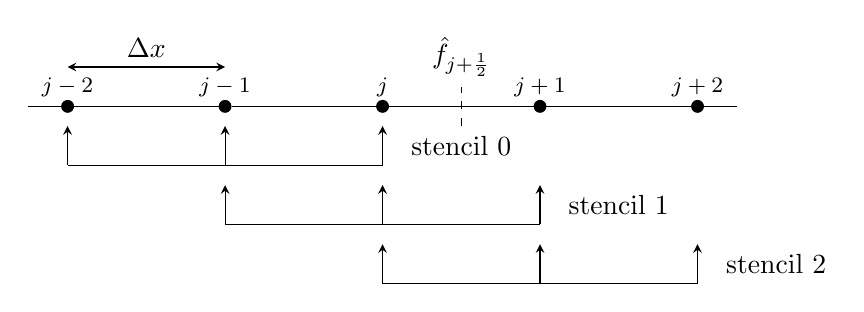
\begin{tikzpicture}
  \stencilpt{-4,0}{j-2}{${j-2}$};
  \stencilpt{-2,0}{j-1}{${j-1}$};
  \stencilpt{ 0,0}{j}  {${j}$};
  \stencilpt{ 2,0}{j+1}{${j+1}$};
  \stencilpt{ 4,0}{j+2}{${j+2}$};
  \draw (j-2) -- (j-1)
        (j-1) -- (j)
        (j)   -- (j+1)
        (j+1) -- (j+2);
  \draw (-4.5,0) -- (j-2)
        ( 4.5,0) -- (j+2);

  \draw[stealth-] (-4,-0.25) -- (-4,-0.75);
  \draw[stealth-] (-2,-0.25) -- (-2,-0.75);
  \draw[stealth-] ( 0,-0.25) -- ( 0,-0.75);
  \draw[-] (-4,-0.75) -- ( 0,-0.75);
  \node[,align=right] at (1,-0.5) {stencil 0};

  \draw[stealth-] (-2,-1) -- (-2,-1.5);
  \draw[stealth-] ( 0,-1) -- ( 0,-1.5);
  \draw[stealth-] (+2,-1) -- (+2,-1.5);
  \draw[-] (-2,-1.5) -- (2,-1.5);
  \node[,align=right] at (3,-1.25) {stencil 1};

  \draw[stealth-] ( 0,-1.75) -- ( 0,-2.25);
  \draw[stealth-] (+2,-1.75) -- (+2,-2.25);
  \draw[stealth-] (+4,-1.75) -- (+4,-2.25);
  \draw[-] (0,-2.25) -- (+4,-2.25);
  \node[,align=right] at (5,-2) {stencil 2};

  \draw[stealth-stealth] (-4,0.5) -- (-2,0.5) node[midway,above] {$\Delta x$};

  \draw[dashed] (1,-0.25) -- (1,0.25) node[above] {$\hat{f}_{j+\frac{1}{2}}$};
\end{tikzpicture}
\end{document}

